\chapter{Progettazione e Implementazione}
\label{cap: design}
%\label{1cap:spinta_laterale}
% [titolo ridotto se non ci dovesse stare] {titolo completo}
%

\begin{citazione}
Vero cuore della tesi, in questo capitolo vengono analizzate nel dettaglio la progettazione e l'implementazione dei due diversi moduli sviluppati. Pur condividendo le stesse finalità, i due moduli implementati presentano caratteristiche ben distinte tra loro. La scelta di tale distinzione deriva in primis dalla volontà di cimentarsi nello sviluppo di un'applicazione che consentisse a un giocatore di fronteggiare una CPU più o meno competitiva in una partita. In secundis, l'analisi delle prestazioni derivante dalla suddetta applicazione avrebbe poi spinto alla creazione di un modello di Machine Learning e al confronto con diversi motori scacchistici, al fine di fornire un'analisi delle prestazioni sempre più accurata e approfondita.
\end{citazione}

\section{Primo Modulo}
L'applicazione è stata realizzata in linguaggio Python. L'intenzione è stata quella di sviluppare un'applicazione utilizzabile da un utente umano per giocare una partita contro un'Intelligenza Artificiale: si è dunque ritenuta opportuna la progettazione di un'interfaccia grafica per l'interazione uomo-macchina. Attraverso la libreria \textit{pygame} è stato possibile creare l'interfaccia in modo programmatico, rappresentando le caselle con array di array di dimensione 8x8 e sfruttando semplici metodi per caricare le immagini dei pezzi precedentemente salvate nella cartella di lavoro. Inoltre, assieme ai pezzi, sono state distinte in maniera visivamente chiara e precisa le caselle chiare da quelle scure. 
\begin{figure}[!htb]
    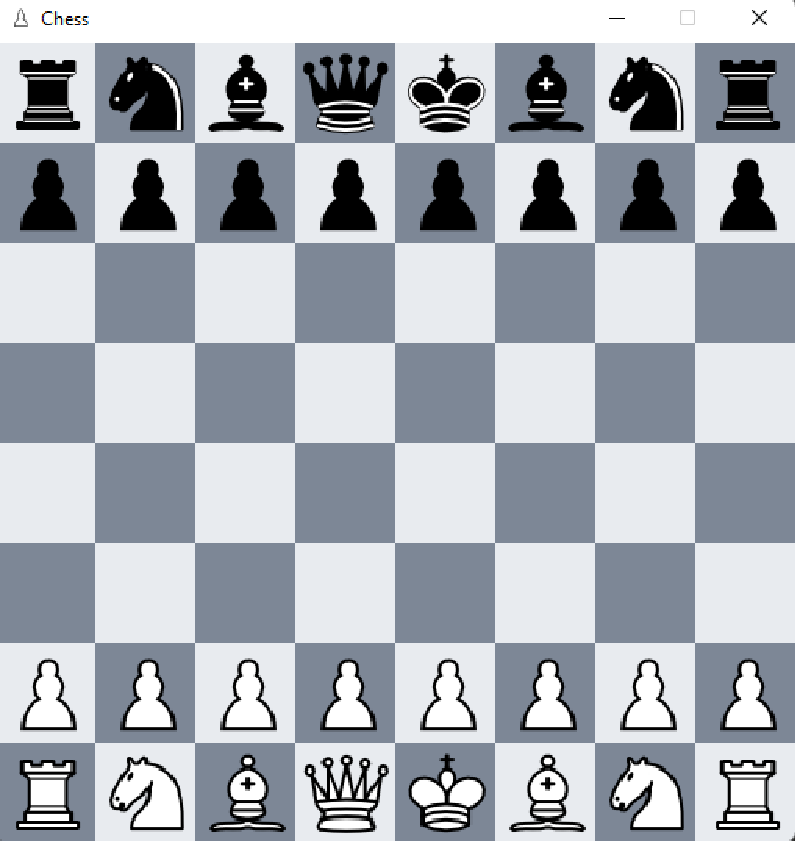
\includegraphics[width=11cm]{frontmatter/figure/scacchiera_gui.pdf}
    \centering
    \caption{Interfaccia grafica vista dall'utente}
    \label{fig:scacchiera_gui}
\end{figure}
\begin{figure}[!htb]
    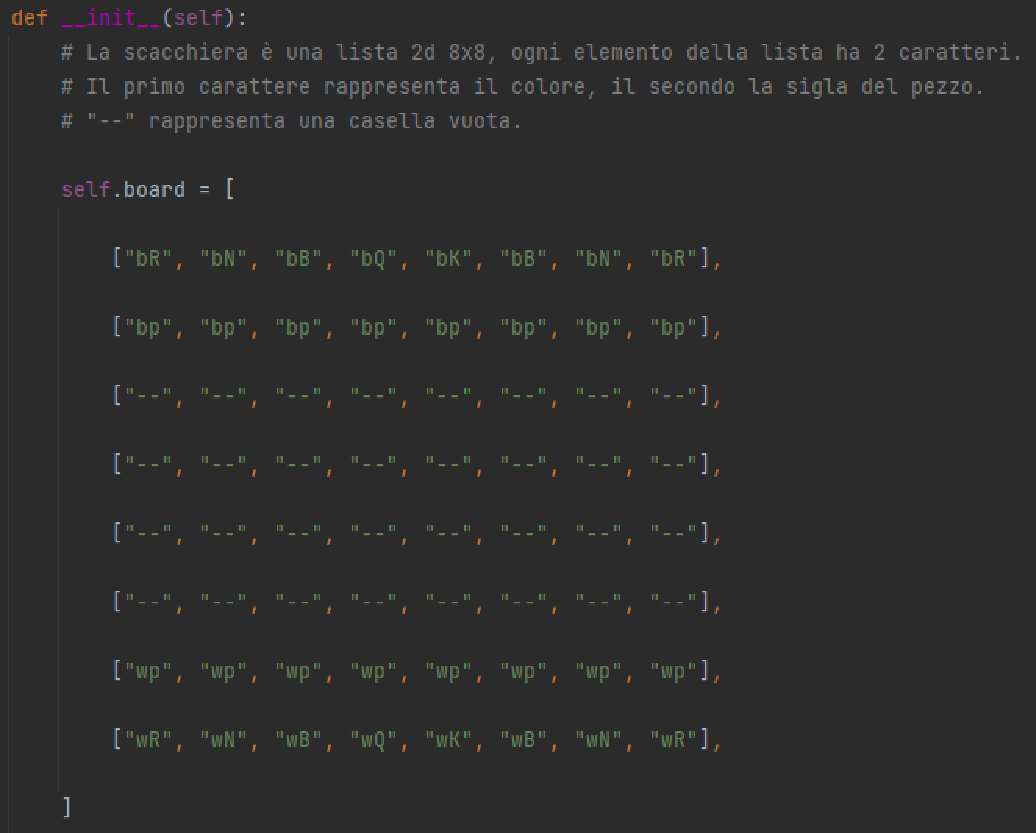
\includegraphics[width=11cm]{frontmatter/figure/rappresentazione_scacchiera.pdf}
    \centering
    \caption{Codifica della figura 3.1}
    \label{fig:rappresentazione_scacchiera}
\end{figure}
\newpage
% Per affiancare due figure
% \begin{figure}[!htb]
% \begin{minipage}[b]{7cm}
% \centering
% 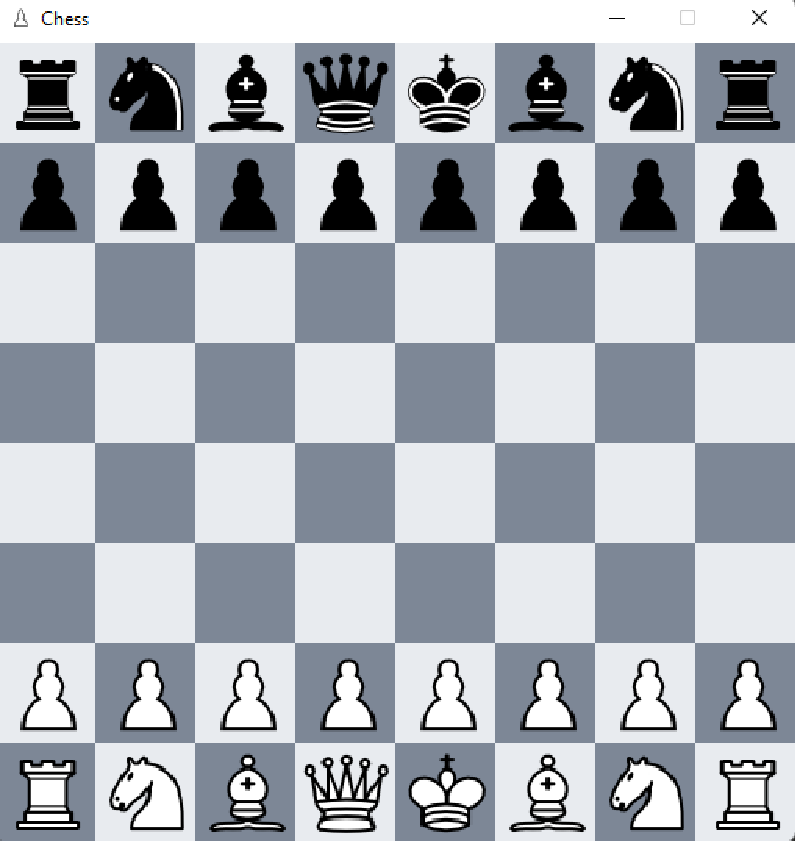
\includegraphics[width=6.5cm]{frontmatter/figure/scacchiera_gui}\\
% \caption{Interfaccia grafica vista dall'utente}
% \label{fig:scacchiera_gui}
% \end{minipage}
% \hspace{1mm}
% \begin{minipage}[b]{7cm}
% \centering
% 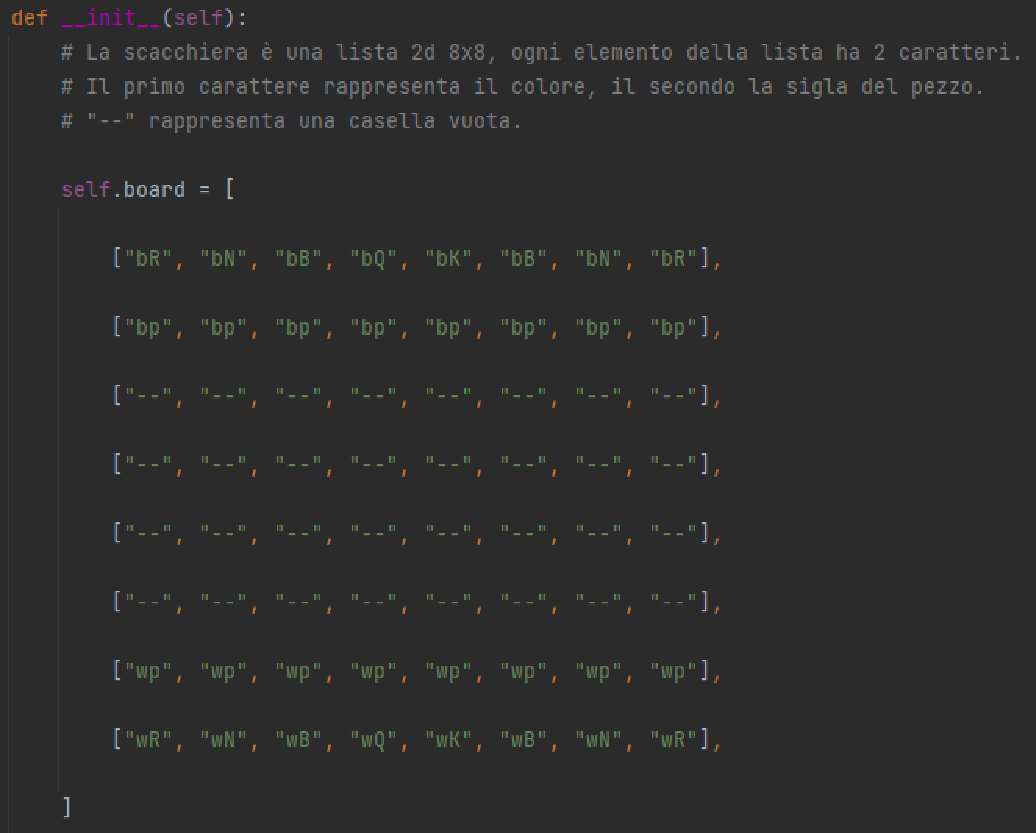
\includegraphics[width=8cm]{frontmatter/figure/rappresentazione_scacchiera}\\
% \caption{Codifica della figura 3.1}
% \label{fig:rappresentazione_scacchiera}
% \end{minipage}
% \end{figure}

A seguito della rappresentazione iniziale della scacchiera sono stati programmati i metodi che si occupano della generazione delle mosse possibili per ciascun pezzo\footnote{Nel gioco degli scacchi il pedone si muove in avanti di una casella (due per la sua prima mossa) e cattura di una casella in diagonale, la torre in orizzontale, l'alfiere in diagonale, il cavallo a L, la regina in orizzontale e in diagonale, e il re di una casella in tutte le direzioni.}, per impedire all'utente di effettuare mosse non legali\footnote{Una mossa non legale è una mossa che pone il re sotto scacco oppure che non libera il re da uno scacco subito nella mossa precedente.}. Analogamente, ad ogni mossa giocata viene effettuato un controllo nel caso in cui il re sia sotto scacco o nel caso in cui vi sia una situazione di scacco matto, dichiarando partita finita nel secondo caso.
\begin{figure}[!htb]
    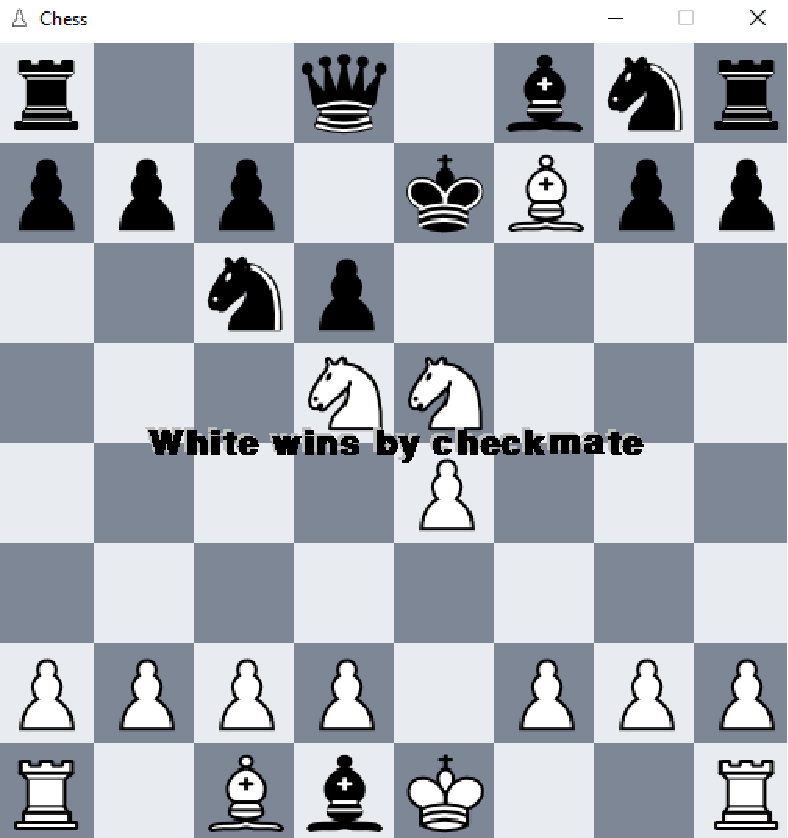
\includegraphics[width=10cm]{frontmatter/figure/checkmate.pdf}
    \centering
    \caption{Partita vinta dal bianco}
    \label{fig:checkmate}
\end{figure}


\subsection{Ricerca delle mosse legali}
Tutta la realizzazione di quanto citato finora è stata effettuata in modo conforme alle tecniche di Intelligenza Artificiale che sono state utilizzate per la generazione delle mosse. L'obiettivo è stato quello di riprogrammare algoritmi di ricerca applicati a una rappresentazione della scacchiera che fosse familiare al programmatore, per comprenderne a fondo il funzionamento. 

\subsubsection{Algoritmo naive}
Una prima, semplice soluzione al problema è stata provata mediante l'utilizzo di un algoritmo naive di ricerca delle mosse. Consideriamo il solito caso in cui il giocatore muove i pezzi bianchi e l'IA i pezzi neri. Dopo una qualsiasi mossa di apertura da parte del bianco, il nero ha un numero molto ristretto di opzioni tra cui scegliere: spostare uno dei pedoni in avanti di una o due caselle, o spostare un cavallo in una delle due caselle legali a inizio partita. Sfruttando un metodo che ritorna la lista di mosse legali data in input una specifica situazione sulla scacchiera, l'algoritmo naive pesca a caso una delle mosse tra quelle disponibili. Chiaramente, un simile approccio sarebbe difficilmente preso in seria considerazione nello sviluppo di un'applicazione del genere, preferendo una soluzione che tenga conto di diversi parametri (mosse storicamente giuste, valore dei pezzi, minacce possibili ai pezzi dell'avversario, trappole in apertura...). Per tale motivo, si è ritenuto necessario lo studio e l'approfondimento di altre metodologie. 

\subsubsection{Algoritmo Greedy}
Nel gioco degli scacchi è fondamentale tenere in considerazione non solo lo stato corrente della scacchiera, ma anche il valore di ciascun pezzo (di solito, un pedone vale molto meno della regina). Sebbene sia vero che talvolta è lo stato stesso della scacchiera a determinare il valore dei pezzi (in alcune situazioni può essere utile sacrificare un pezzo di valore alto per vincere la partita), per convenzione si è deciso di assegnare a ciascun pezzo un valore intero di default. Questi valori sono sfruttati in un metodo di valutazione dello stato corrente della scacchiera, che indica quanto la situazione in corso sia più o meno favorevole per la vittoria.
\begin{figure}[!htb]
    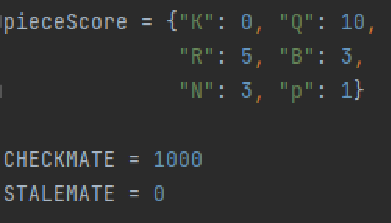
\includegraphics[width=10cm]{frontmatter/figure/valore_pezzi.pdf}
    \centering
    \caption{Valore dei pezzi, scacco matto e stallo}
    \label{fig:valore_pezzi}
\end{figure}\\

Più preciso e affidabile dell'algoritmo precedentemente considerato, l'algoritmo greedy tende più a mettere in difficoltà l'avversario piuttosto che a vincere la partita, spesso in maniera controproducente. La priorità di questa strategia è infatti quella di catturare i pezzi dell'avversario, anche a costo di mettere a rischio i propri. In ogni caso, è interessante notare come, tenendo in considerazione il valore dei pezzi, quest'algoritmo favorisca la cattura di pezzi "pesanti" piuttosto che di altri. 
\subsubsection{Algoritmo minimax}
La strategia minimax è una soluzione studiata appositamente per i giochi a somma zero, come nel caso degli scacchi. Lo scopo, come suggerisce il nome, è quello di \textbf{minimizzare la massima perdita} possibile, analizzando l'albero delle decisioni e valutando l'utilità di un nodo di trovarsi nello stato corrente (a patto che entrambi i giocatori scelgano mosse ottime fino alla fine della partita). A differenza dei due algoritmi precedentemente analizzati, dunque, salta subito all'occhio la prima peculiarità dell'algoritmo, che tiene in stretta considerazione le mosse dell'avversario e gioca comportandosi di conseguenza. Attraverso l'algoritmo minimax il problema di ricerca della mosse migliore è stato ridotto al problema della visita dell'albero delle decisioni. Analizzando la complessità intrinseca del gioco degli scacchi trattata nei capitoli precedenti si è ritenuto necessario effettuare una leggera modifica all'algoritmo minimax che tenesse in considerazione la profondità con cui scendere nell'albero, portando il problema a livelli più o meno trattabili in termini di complessità temporale (l'analisi nel dettaglio delle prestazioni è rimandata al paragrafo \ref{cap: Analisi}).
\subsubsection{Algoritmo negamax con potatura alfa-beta}
% citare wikipedia
L'algoritmo negamax costituisce una variante dell'algoritmo minimax. La caratteristica principale dell'algoritmo è quella di considerare il valore del giocatore A in un certo gioco come la negazione del valore del giocatore B. Così, il giocatore che deve muovere cercherà una mossa che massimizzi la negazione del valore della posizione risultante dalla mossa: così facendo, basta un singolo calcolo per ricavare il valore di tutte le posizioni. Questa è chiaramente una semplificazione rispetto al minimax. Un'ulteriore miglioria all'algoritmo è stata apportata considerando la \textbf{potatura alfa-beta}. L'idea è in realtà applicabile a qualsiasi albero, e consente di ridurre significativamente la complessità di tempo necessaria all'esplorazione. Consideriamo un qualsiasi nodo \textit{n} raggiungibile: se esiste un'alternativa \textit{m} migliore, allora \textit{n} e tutti i suoi discendenti non saranno mai esplorati, portando a una vera e propria "potatura" dell'albero. L'efficacia dell'algoritmo, in ogni caso, dipendente dall'ordinamento dei nodi visitati, che dipende da gioco a gioco. Nel caso degli scacchi, sarebbe una buona idea considerare dapprima le mosse che catturano i pezzi avversari, poi le mosse che li minacciano e infine le altre. 

\subsection{Analisi delle prestazioni}
\label{cap: Analisi}
Non è stata fornita un'analisi delle prestazioni per tutti gli algoritmi discussi finora. Le forti limitazioni di alcune delle strategie adottate per risolvere il problema della ricerca di una mossa non hanno favorito un'interesse significativo: la "casualità" a cui si affida l'algoritmo naive e la bassa considerazione delle mosse dell'avversario dell'algoritmo Greedy non consentirebbero un'indagine interessante. Al contrario, data la natura della strategia minimax che si serve di un vero e proprio albero di ricerca in cui ciascun nodo rappresenta una mossa legale, si è ritenuto opportuno procedere all'analisi prestazionale del suddetto algoritmo. Per sua natura, l'algoritmo minimax non è efficiente in termini di complessità temporale: essendo essa governata dalla dimensione \textit{m} dell'albero, nel caso peggiore la ricerca avrà complessità $O(b^m)$.

\begin{table}[!htb]
    \centering
    \begin{tabular}{|c|c|c|c|}
\hline
\textbf{Profondità} & \textbf{Prima Mossa} & \textbf{Seconda Mossa} & \textbf{Terza Mossa}\\
\hline
\textbf{1} & 0,26 & 0,56 & 0,94\\
\hline
\textbf{2} & 1,39 & 3,02 & 4,02\\
\hline
\textbf{3} & 41,74 & 82,96 & 192,34\\
\hline
\end{tabular}
    \caption{Tempo di visita dell'albero (in secondi) al variare della profondità (senza potatura)}
    \label{tab:my_label}
\end{table}

Tempi del genere rendono il problema intrattabile. Si notano sin da subito, a una profondità non eccessivamente elevata, i tempi d'attesa per la ricerca dopo appena la terza mossa, che in una partita di circa venti o trenta mosse sarebbero notevolmente elevati. Per ovviare al problema è stata aggiunta la tecnica della \textbf{potatura}, che consente di evitare di visitare tutti i nodi dell'albero, alla variante negamax. I risultati delle prestazioni dell'algoritmo negamax con potatura alfa-beta sono forniti di seguito.

\begin{table}[!htb]
    \centering
    \begin{tabular}{|c|c|c|c|}
\hline
\textbf{Profondità} & \textbf{Prima Mossa} & \textbf{Seconda Mossa} & \textbf{Terza Mossa}\\
\hline
\textbf{1} & 0,15 & 0,19 & 0,35\\
\hline
\textbf{2} & 0,86 & 1,32 & 2,85\\
\hline
\textbf{3} & 11,74 & 17,77 & 59,81\\
\hline
\end{tabular}
    \caption{Tempo di visita dell'albero (in secondi) al variare della profondità (con potatura)}
    \label{tab:my_label}
\end{table}

La complessità esponenziale dell'algoritmo permane, ma si può notare dai dati un andamento sostanzialmente "meno esponenziale" dell'algoritmo precedentemente adottato.

\subsection{Migliorie della funzione di valutazione}
A seguito dell'analisi degli algoritmi sono stati effettuati degli esperimenti sul funzionamento delle tecniche di Intelligenza Artificiale apportando modifiche al metodo di valutazione della posizione sulla scacchiera. Come indicato nel paragrafo dedicato all'algoritmo Greedy era stato originariamente considerato un dizionario che tenesse traccia del valore di ciascun pezzo, ottenendo un valore più alto per un pezzo come la Regina piuttosto che per un pedone. Questo paragrafo è invece dedicato alla descrizione di una nuova funzione di valutazione, che tiene traccia non solo del valore di un pezzo, ma anche dell'utilità della sua posizione sulla scacchiera.

\begin{figure}[!htb]
    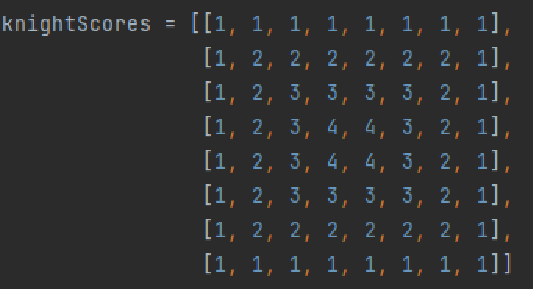
\includegraphics[width=9cm]{frontmatter/figure/cavallo.pdf}
    \centering
    \caption{Utilità delle caselle per il cavallo}
    \label{fig:valore_cavallo}
\end{figure}

\begin{figure}[!htb]
    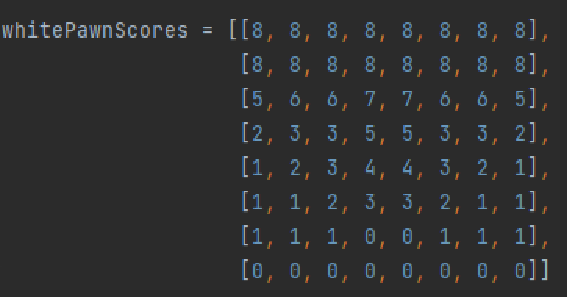
\includegraphics[width=9cm]{frontmatter/figure/pedone.pdf}
    \centering
    \caption{Utilità delle caselle per il pedone bianco}
    \label{fig:valore_pedoni}
\end{figure}
\newpage
Come indicato dalla \textbf{figura \ref{fig:valore_cavallo}} l'utilità del cavallo di trovarsi in una certa casella è stata valutata con un intero da 1 a 4 in base alla "minaccia" che è possibile portare avanti in quella posizione: un cavallo mantenuto verso il centro della scacchiera è chiaramente più forte di un cavallo mantenuto verso i bordi, essendo in quest'ultimo caso più limitato nei movimenti. Analogamente, le posizioni considerate per il pedone bianco nella \textbf{figura \ref{fig:valore_pedoni}} suggeriscono un'idea simile: per un pedone è importante non solo controllare le caselle in diagonale, ma anche cercare di arrivare al lato opposto della scacchiera (al quale è assegnato il valore più alto) per arrivare a promozione. 

\subsubsection{Cambiamenti nelle prestazioni}
Sebbene sia stata apportata una modifica alla funzione di valutazione, la complessità dell'algoritmo di ricerca non è variata in modo significativo. Il motivo è da ricercare, come già spiegato nel paragrafo dedicato, alla natura intrinseca dell'algoritmo. Le costanti migliorie apportate alla funzione di valutazione non sarebbero abbastanza per ridurre i tempi di visita dell'albero delle decisioni. Una riduzione notevole dei tempi di esecuzione era stata già ottenuta attraverso la tecnica della potatura alfa-beta.

\section{Secondo Modulo - Caissa}
La modifica della funzione di valutazione del primo modulo gettava le basi per la ricerca di una metodologia completamente nuova, tenendo a mente le motivazioni e gli obiettivi del lavoro in corso. La volontà di raccogliere i risultati del modulo precedentemente discusso e di evitare di fornire nuovi algoritmi la cui discussione sarebbe stata ridondante si è dunque tradotta nell'intenzione di trattare il problema del gioco degli scacchi da un approccio differente. In questa seconda parte del capitolo si esaminano vere e proprie tecniche di \textbf{Machine Learning}, che sono state sperimentate in un modulo tutto nuovo. I risultati si sono tradotti nella creazione di \textbf{Caissa}, un motore scacchistico in grado di comprendere lo stato della scacchiera e giocare di conseguenza.
\newpage
\subsection{Machine Learning e reti neurali artificiali}
La teoria dell'apprendimento è quella branca dell'Intelligenza Artificiale che si occupa, per l'appunto, dell'apprendimento degli agenti intelligenti, permettendogli di operare in ambienti inizialmente sconosciuti in maniera sempre più appropriata. Tale miglioramento viene effettuato attraverso l'operato stesso dell'agente, dunque in base all'esperienza, ma ciò non preclude necessariamente all'agente di imparare per mezzo di dati che gli sono stati forniti in input.
Uno degli aspetti maggiormente considerati nel contesto analizzato nel lavoro di tesi è quello del \textbf{Deep Learning}: sono state infatti sfruttate tecniche basate su vere e proprie \textbf{reti neurali\footnote{In Biologia, una rete neurale è un gruppo di neuroni che svolgono una determinata funzione fisiologica.} artificiali} organizzate in diversi strati, dove ogni strato scambia le informazioni con quello successivo per garantire un'elaborazione dell'informazione sempre più accurata. Per le tipologie di dati da elaborare le tecniche di Machine Learning adottate si servono di reti neurali \textbf{convoluzionali}, essendo queste particolarmente adatte per l'elaborazione di dati di tipo 2D.

\subsection{Preparazioni preliminari alla fase di addestramento}
Per lo sviluppo del modulo è stata abbandonata l'implementazione precedentemente programmata, favorendo l'utilizzo di una API in linguaggio Python: le esigenze hanno portato alla ricerca di un'implementazione che fosse stabile, completa, e continuamente supportata e manutenuta dagli sviluppatori. Inoltre, è stata utilizzata piattaforma \textbf{Jupyter Notebook}, utile al programmatore per visionare in maniera chiara e user friendly i pezzi sulla scacchiera. Attraverso l'ausilio della piattaforma \textbf{Colab} di Google è stato recuperato il dataset da dare in input al modello di rete neurale per l'addestramento, contenente milioni di partite di scacchi, ciascuna col proprio log delle mosse giocate. L'obiettivo è stato infatti quello di valutare partite note e addestrare il modello a giocare in modo competitivo proprio considerando quelle partite. La valutazione delle posizioni fornite in input è stata effettuata mediante il motore \textit{Stockfish 15} che, sulla base di diversi parametri come ad esempio il vantaggio materiale, la sicurezza del proprio re, la coordinazione dei propri pezzi e diversi altri fattori, fornisce in output un intero positivo (vantaggio del bianco) o negativo (vantaggio del nero).\newpage

\begin{figure}[!htb]
    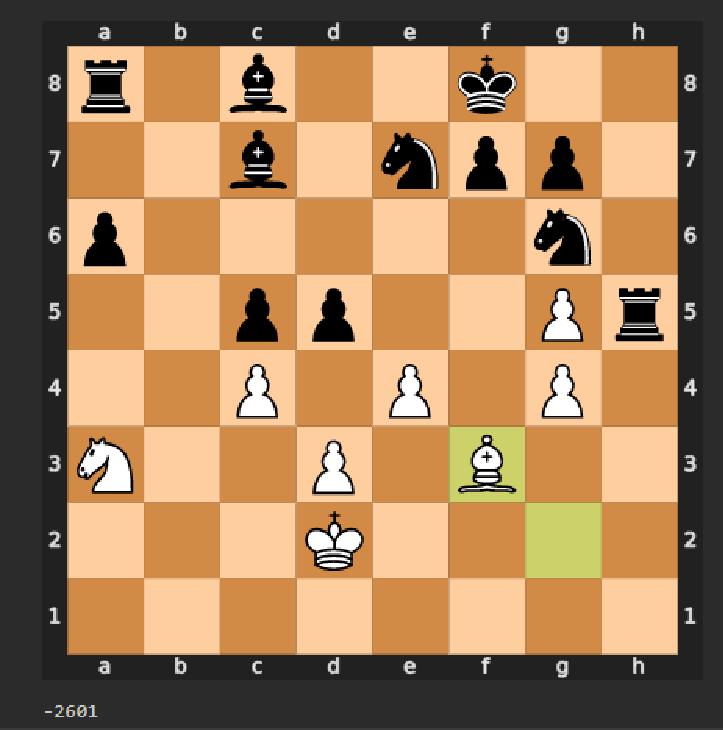
\includegraphics[width=10cm]{frontmatter/figure/valutazione_scacchiera.pdf}
    \centering
    \caption{Vantaggio materiale e posizionale del nero con rispettivo punteggio}
    \label{fig:valutazione_scacchiera}
\end{figure}

La rappresentazione della scacchiera è stata presa e rielaborata per il problema in questione, rendendola più adatta alla rete neurale convoluzionale che sarebbe stata usata in seguito. Nello specifico, è stata adottata una matrice 3D che rappresentasse le caselle e il tipo dei pezzi.

\subsection{Costruzione del modello e addestramento}
Stabiliti gli ambienti favorevoli ha avuto inizio il lavoro vero e proprio, durante il quale Caissa è stato creato e addestrato. Lo sviluppo è avvenuto con \textbf{Keras}, una libreria in Python adatta per l'apprendimento automatico e la creazione di modelli di rete neurale. Dopo aver costruito il tensor sulla base della rappresentazione della scacchiera precedentemente descritta, sono stati aggiunti i layers convoluzionali per la trasmissione delle informazioni. L'addestramento è stato in seguito effettuato sulla base del dataset menzionato nel paragrafo precedente. Infine, è stato implementato un algoritmo minimax di ricerca delle mosse: sebbene si tratti di una soluzione adottata anche nella stesura del primo modulo è interessante notare che, nonostante la differenza di background, la strategia minimax si sia rivelata adatta anche per il funzionamento di un modello di rete neurale.

\subsection{Punteggio ELO e valutazione del modello}
Nell'ambito dei giochi a somma zero è diffuso il metodo di valutazione \textbf{ELO} per calcolare le abilità di un giocatore. Si tratta sostanzialmente di un numero il cui valore aumenta o diminuisce a seconda della vittoria o della sconfitta di una partita contro un altro avversario.
Per la valutazione delle performance di Caissa, dunque, non è stata effettuata un'analisi da un punto di vista computazionale come era stato fatto per il primo modulo. Questo perché eventuali migliorie da apportare a Caissa sarebbero pensate per migliorare la sua performance sportiva: pertanto, è stato scelto un approccio "ad alto livello" sulla base di diverse partite giocate contro altri motori scacchistici preparati dal programmatore. I primi (pochi) incontri sono stati giocati contro il motore \textit{Stockfish 13}. L'intenzione era quella di fissare un upper bound della valutazione di Caissa, essendo \textit{Stockfish} uno dei migliori motori scacchistici moderni con un ELO di circa 3546 alla versione considerata. 
% citare https://www.ichess.net/blog/best-chess-engines/
Come previsto, \textit{Stockfish} ha avuto la meglio in tutte le partite disputate. Partite più eque sono state giocate contro motori scacchistici con un punteggio ELO stimato che varia tra i 500 e i 1200. Nello specifico, sono stati considerati tre modelli: Alpha (512), Beta (870) e Gamma (1190). Nella sua prima versione, in realtà, il punteggio ELO di Caissa è stato stimato al di sotto dei 500 punti, essendo stato battuto persino da Alpha. Nel prossimo capitolo verranno discusse diverse idee che potrebbero essere applicate per migliorare le prestazioni di Caissa e aumentare il suo punteggio.



\newpage
